% IEEE Transactions revision. All numbers in Sections VI-VII are generated from results/v2/*.csv
% (tools/make_v2_tables.py, tools/make_v2_figures.py) of the Satellite_Optical_GitHub_Publish project.
\documentclass[journal]{IEEEtran}
\usepackage[utf8]{inputenc}
\usepackage[T1]{fontenc}
\usepackage{amsmath,amssymb,amsthm}
\usepackage{graphicx}
\usepackage{booktabs}
\usepackage{array}
\usepackage{cite}
\usepackage{url}
\usepackage[hidelinks]{hyperref}

\DeclareMathOperator{\Log}{Log}
\DeclareMathOperator{\Exp}{Exp}
\DeclareMathOperator{\sat}{sat}
\DeclareMathOperator{\clip}{clip}
\newcommand{\urad}{\,\mu\text{rad}}
\newtheorem{lemma}{Lemma}
\newtheorem{theorem}{Theorem}
\newtheorem{corollary}{Corollary}
\newtheorem{remark}{Remark}
\newtheorem{assumption}{Assumption}

\begin{document}

\title{Certified Link-Aware Attitude Coordination of Spacecraft Under Physically Modelled Optical-Link Degradation}

\author{C.~Rishitha, Y.~Karthikeya, A.~Tyagi, S.~Kaushal, and R.~Satheesh%
\thanks{The authors are with the Amrita School of Artificial Intelligence, Amrita Vishwa Vidyapeetham, Coimbatore, India.}}

\maketitle

\begin{abstract}
In leader-following attitude coordination over optical crosslinks, a pointing fault or outage removes the neighbor states that followers need, and conventional triggering rules cannot tell how much that loss costs. This paper proposes Certified Link-Aware Coordination (CLAC). Every spacecraft carries an online bound on its attitude and rate error against the true desired attitude. Packets carry the bound; a receiver grows it with the packet age using only the command-generator class constants. We prove that the bound holds under arbitrary delay, loss and outage, without assuming a stable closed loop. CLAC uses the bound to set the extrapolation horizon and to re-select its parent among all other spacecraft. The optical layer is a physical model: link budget, receiver noise, bit-error rate, Reed--Solomon packet errors, a lock and acquisition state machine, terminal lag and tracking jitter. The link-budget code reproduces the published NASA TBIRD downlink budget to 0.07~dB. Nine methods, including static, dynamic and self-triggered baselines tuned on separate seeds to a matched payload, are compared on 2{,}520 held-out runs: 14 conditions, including an isolated actuator fault, pointing bias on one, three and six links, and random single- and two-link outages. Over the 14 conditions CLAC lowers fault-window pair error by 58.4\% (95\% CI: $[55.8, 61.2]\%$) relative to a leader-fed event-triggered star, at 14.5\% more payload. It ties the best baseline when no link fails and gains most under link outages. The certificate was never violated in 560 CLAC runs. Closed-loop stability of the saturated controller is not proved, and no raw NASA or ISRO telemetry is used.
\end{abstract}

\begin{IEEEkeywords}
Spacecraft attitude coordination, optical inter-satellite links, event-triggered control, certified error bound, fault tolerance, networked control.
\end{IEEEkeywords}

\section{Introduction}
Optical crosslinks let small spacecraft exchange state at high rate, but they couple communication to attitude: body motion changes terminal pointing, pointing changes received power, and power decides whether packets arrive~\cite{click}. In leader-following coordination only one spacecraft receives the moving command, so a lost link leaves followers extrapolating a stale neighbor state~\cite{cai2014,dimarogonas2009}. Event-triggered and self-triggered schemes reduce traffic when links work~\cite{tabuada2007,heemels2012,girard2015,xie2023,xie2024taes,wang2021,jia2023}, but they decide \emph{when to send}. They do not tell a receiver how wrong its target may be after a long silence, and they assume a fixed communication tree.

This paper addresses that gap. Its contributions are:
\begin{enumerate}
\item \textbf{A certificate.} An online-computable bound on each follower's attitude and rate error against the true desired attitude, carried in packets and grown with message age by the command-generator constants (Lemma~\ref{lem:ext}, Theorem~\ref{thm:cert}). It is valid for arbitrary delays, losses and outages and for any parent selection. It does not assume closed-loop stability or acceleration bounds on the follower.
\item \textbf{CLAC.} A coordination rule that uses the certificate for decisions: a certified extrapolation horizon, decentralised re-selection of the parent with the smallest certified bound (with hysteresis), and lock-aware link scheduling (Section~\ref{sec:clac}).
\item \textbf{A physical optical layer validated against published NASA data.} A link budget, receiver, coding, lock and terminal model replaces the earlier Gaussian power threshold. The budget code reproduces the NASA/MIT Lincoln Laboratory TBIRD downlink budget to 0.07~dB, and beam width, jitter and pull-in time are taken from the same publications (Section~\ref{sec:optics}).
\item \textbf{A broader, stricter evaluation.} Nine methods, 14 conditions and 2{,}520 held-out runs on seeds never used before, with budget-matched baselines, an isolated actuator fault, pointing bias on one, three and six links, random single- and two-link outages, a hash-locked protocol and an independent recomputation (Section~\ref{sec:protocol}).
\end{enumerate}
The scope is simulation. The results do not establish flight performance or closed-loop stability, and they rely on adapted versions of published triggering rules, not their authors' code. Section~\ref{sec:limits} lists what is not shown.

\section{Related Work}
\emph{Attitude coordination and triggered communication.} Leader-following and synchronisation laws for rigid bodies are well studied~\cite{ren2007,sarlette2009,abdessameud2009,mayhew2011,dimarogonas2009,cai2014}. Event-triggered attitude and formation schemes with delays, saturation, faults or learning terms appear in~\cite{wang2021,xie2023,xie2024asr,jia2023,xie2024taes}, building on static event triggering~\cite{tabuada2007}, periodic and self-triggered variants~\cite{heemels2013,mazo2010,heemels2012,donkers2012} and the dynamic trigger with an internal variable~\cite{girard2015}. These works prove stability of their own closed loops under their assumptions; in all of them the receiver holds or extrapolates the last message. To the best of our knowledge, within the literature we reviewed, none propagates a certified error bound with the message, uses it to choose among neighbours, and evaluates the result over a physically modelled optical link. This is a statement about the sources we found, not a proof of absence.

\emph{Networked control.} Delays, losses and intermittent observations are covered in~\cite{hespanha2007,zhang2001,sinopoli2004,olfati2007,nowzari2019}. Our certificate does not compete with these stability analyses; it bounds a different quantity, the error of the neighbour-derived target, and only needs a bounded command class.

\emph{Optical links.} Surveys cover acquisition, tracking and pointing~\cite{kaymak2018,kaushal2017,toyoshima2005}, and free-space pointing-error and outage analyses~\cite{farid2007,khalighi2014}. NASA and MIT Lincoln Laboratory published detailed on-orbit results for the TBIRD downlink~\cite{schieler2023,schieler2023icsos}. We use these published values to calibrate and check the link-budget arithmetic; we do not claim that a crosslink at 1~km behaves like a 930~km downlink.

\emph{Fault diagnosis.} Fault-tolerant control separates diagnosis from accommodation~\cite{zhang2008}, and active diagnosis designs probing inputs~\cite{heirung2019,scott2014,raimondo2016}. Our terminals use a fixed pilot dither and a Gaussian power fit, not an optimised input.

\section{System Model}
\subsection{Attitude, Reference and Information Structure}
For spacecraft $i\in\{1,\dots,4\}$, $q_i$ is a scalar-first unit quaternion, $R(q)$ its rotation matrix, $\otimes$ quaternion product, $\Exp,\Log$ the rotation-vector maps, and
\begin{align}
\dot q_i &= \tfrac12 q_i\otimes[0,\omega_i^T]^T,\\
J\dot\omega_i &= D_{\eta_i}u_i+d_i-\omega_i\times J\omega_i,
\end{align}
with $J=\mathrm{diag}(0.030,0.025,0.020)$~kg\,m$^2$, torque bound $0.002$~N\,m per axis, disturbance $d_i$, and diagonal actuator effectiveness $D_{\eta_i}$. The four spacecraft sit at the corners of a 1000~m square (six physical links). The reference $q_r(t)=\Exp(v_r(t))$ with $v_r=[.018\sin(.11t+p),\,.012\sin(.07t+.4+p),\,.010\sin(.09t-.2+p)]^T$~rad has body rate $\omega_r$. Constant offsets $o_i$ give the desired attitude and rate of spacecraft $i$,
\begin{equation}
q_i^\star=q_r\otimes o_i,\qquad \omega_i^\star=R(o_i)^T\omega_r .
\end{equation}
Only SC1 receives $q_r$. Followers derive a \emph{target} $(q_{t,i},\omega_{t,i})$ from a delivered neighbour packet. Local feedback is a saturated PD-plus-sliding term with a disturbance estimate~\cite{liu2018}; it is identical for all methods and its closed loop is not analysed here.

\begin{assumption}[Command class]\label{as:ref}
$\|\omega_r(t)\|\le\bar\omega$ and $\|\dot\omega_r(t)\|\le\bar\alpha$ for all $t$, and $\bar\omega,\bar\alpha$ are known to every spacecraft.
\end{assumption}
For the command above, a dense numerical check over 25 phases and 200~s gives $\max\|\omega_r\|=2.31\times10^{-3}$ and $\max\|\dot\omega_r\|=2.38\times10^{-4}$, so $\bar\omega=2.45\times10^{-3}$~rad/s and $\bar\alpha=2.6\times10^{-4}$~rad/s$^2$ are used (checked in \texttt{tests/test\_certificate.m}).

\subsection{Packets and Delivery}
Directed endpoint $a:i\to j$ sends packets containing the sender's quaternion, rate, timestamp and, for CLAC, two bounds and a parent index. A baseline packet is 64~B (eight doubles) and a CLAC packet 88~B. A packet is lost with the packet-error probability of the optical layer (Section~\ref{sec:optics}), delayed by $0.10+0.10U$~s ($U$ uniform), and accepted only if its timestamp is newer than the cache. There are 32 queue slots per endpoint, and a packet is discarded when the link is unlocked at arrival. The network-transfer condition adds a 10\% extra loss floor. All methods see the same random draws on the same seed.

\section{Physical Optical Layer}\label{sec:optics}
\subsection{Link Budget, Receiver and Coding}
The received power of endpoint $a$ is
\begin{equation}
P_a=P_{0,a}\,G_a\,\exp\!\Big(-\frac{2\|x_a+b_a+\xi_a\|^2}{\alpha^2}\Big),
\end{equation}
with residual pointing $x_a$, hidden bias $b_a$, tracking jitter $\xi_a\sim\mathcal N(0,\sigma_\xi^2 I)$, attenuation $G_a$, and $1/e^2$ half-angle $\alpha=\mathrm{FWHM}/\sqrt{2\ln2}$. The nominal power $P_{0}$ follows from
\begin{equation}
P_0=\underbrace{P_t L_t}_{\text{Tx}}\ \underbrace{\tfrac{16\ln2}{\mathrm{FWHM}^2}}_{G_t}\ \underbrace{\tfrac{1}{4\pi r^2}}_{\text{range}}\ \underbrace{A_rL_r}_{\text{Rx}},
\end{equation}
which for $P_t=5$~mW, $L_t=-1$~dB, FWHM $=380\urad$, a 10~mm aperture, $L_r=-5.2$~dB and $r=1$~km gives $P_0=0.576\,\mu$W and $\alpha=322.7\urad$ (Table~\ref{tab:optics}). The receiver is a PIN photodiode with a transimpedance front end (thermal, shot and background noise) and on-off keying, giving the bit-error rate $\mathrm{BER}=\tfrac12\mathrm{erfc}(Q/\sqrt2)$ with $Q=I_1/(\sigma_0+\sigma_1)$. A shortened Reed--Solomon code RS(88,72) over GF$(2^8)$ corrects $t=8$ symbols~\cite{reed1960}, so a codeword (packet) is lost with probability $\sum_{k>t}\binom{n}{k}p_s^k(1-p_s)^{n-k}$, where $p_s=1-(1-\mathrm{BER})^8$. The link-availability threshold is not an input: it is the power where the packet error equals 0.1, $0.112\,\mu$W ($-39.5$~dBm), leaving a nominal margin of 7.1~dB. Fig.~\ref{fig:receiver} shows both error curves.

\begin{figure}[!t]
\centering
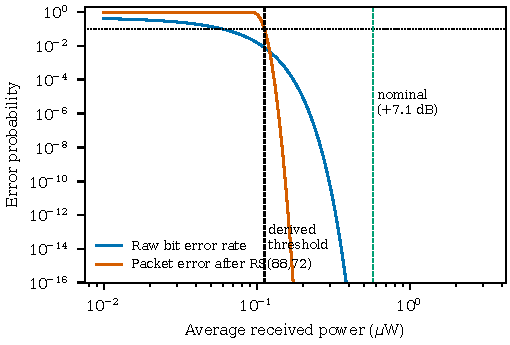
\includegraphics[width=\columnwidth]{figures/fig_v2_receiver.pdf}
\caption{Receiver model: raw bit-error rate and packet error after RS(88,72) versus average received power. The dashed lines mark the derived availability threshold and the nominal operating power.}
\label{fig:receiver}
\end{figure}

\subsection{Lock, Acquisition and Terminal Dynamics}
Each terminal tracks only while power stays above the threshold. A lock is lost after 0.5~s below it. Re-acquisition requires power at least 1.5 times the threshold for an acquisition dwell (3~s nominal, 15~s in a stress case), and a link carries packets only when both terminals are locked. The terminal is two cascaded 0.03~s lags with a 0.035~rad/s rate limit, tracking jitter $\sigma_\xi=10\urad$ RMS (35~$\mu$rad in a stress case), and encoder noise of $5\urad$. A local pilot dither and a Gaussian power fit estimate boresight bias as before; the fit-acceptance residual (0.20) was set on development seeds.

\begin{table}[!t]
\caption{Optical-layer parameters and their provenance}
\label{tab:optics}
\centering\footnotesize
\begin{tabular}{@{}p{0.40\columnwidth}p{0.52\columnwidth}@{}}
\toprule
Parameter & Value (source)\\
\midrule
Beam FWHM & $380\urad$ (NASA TBIRD, on-orbit measurement~\cite{schieler2023})\\
Body pointing jitter & $<10\urad$ RMS nominal~\cite{schieler2023icsos}; $35\urad$ stress (20--35~$\mu$rad uplink tracking~\cite{schieler2023})\\
Pull-in time & 3~s nominal (assumed); 15~s stress (TBIRD 10--30~s~\cite{schieler2023})\\
Tx power / losses & 5~mW; $-1$~dB Tx, $-5.2$~dB Rx (design, assumed)\\
Receiver, code & responsivity 0.9~A/W, 5~pA/$\sqrt{\text{Hz}}$, 100~Mbps OOK; RS(88,72) (design)\\
Lock hysteresis & 0.5~s loss hold, $1.5\times$ re-acquire (assumed)\\
Derived threshold & 0.112~$\mu$W at packet error 0.1\\
\bottomrule
\end{tabular}
\end{table}

\subsection{Validation Against Published NASA Data}
Table~\ref{tab:tbird} reproduces the downlink irradiance budget published for TBIRD at $30^\circ$ elevation~\cite{schieler2023} with the same budget function the crosslink simulator calls. The model total of $-52.97$~dB\,W/m$^2$ differs from the published $-52.9$ by 0.07~dB, and no line item differs by more than 0.15~dB.

\begin{table}[!t]
\caption{TBIRD downlink irradiance budget: published~\cite{schieler2023} versus the simulator's budget code}
\label{tab:tbird}
\centering\footnotesize
\begin{tabular}{@{}lrrr@{}}
\toprule
Item & Published & Model & Diff.\\
\midrule
Tx optical power, 0.9~W (dBW) & $-0.5$ & $-0.46$ & 0.04\\
Tx optics loss (dB) & $-0.3$ & $-0.30$ & 0.00\\
Tx gain, 380~$\mu$rad (dBi) & 79.0 & 78.85 & $-0.15$\\
Pointing loss, 50~$\mu$rad (dB) & $-0.2$ & $-0.21$ & $-0.01$\\
Range loss, 930~km (dB/m$^2$) & $-130.4$ & $-130.36$ & 0.04\\
Atmospheric loss (dB) & $-0.5$ & $-0.50$ & 0.00\\
\midrule
Irradiance (dB\,W/m$^2$) & $-52.9$ & $-52.97$ & $-0.07$\\
\bottomrule
\end{tabular}
\end{table}

\emph{What is real and what is modelled.} The budget, beam width, jitter range, pull-in range and the existence of a hard FEC threshold (about $-38$~dBm in the 200~Gbps mode) are published NASA/MIT-LL values. The 1~km crosslink geometry, the 100~Mbps receiver, the RS code, the lock thresholds and the transmitter power are modelled. Raw flight telemetry from NASA is not public, and we found no public ISRO inter-satellite-link data, so none is used. The validation therefore tests the link-budget arithmetic and calibrates the model; it is not a validation of the whole closed loop against flight data.

\section{Certified Link-Aware Coordination}\label{sec:clac}
\subsection{Certificate}
For spacecraft $i$ define the attitude and transported rate errors against the true desired state,
\begin{equation}
\chi_i=\|\Log(q_i^{\star*}\!\otimes q_i)\|,\quad
\epsilon_i=\|\omega_i-R(q_i)^TR(q_i^\star)\omega_i^\star\|.
\end{equation}
Let a packet from $j$ stamped $\tau$ carry $(q_j,\omega_j)$ and bounds $\chi_j\le H$, $\epsilon_j\le W$ at $\tau$. Spacecraft $i$ forms, at $t=\tau+a$, the target
\begin{equation}
\begin{aligned}q_{t}(a)&=q_j\otimes\Exp(\omega_j\min(a,h))\otimes\rho,\\ \omega_{t}&=\begin{cases}R(\rho)^T\omega_j,&a<h\\ 0,&a\ge h\end{cases}\end{aligned}
\end{equation}
with $\rho=o_j^*\otimes o_i$ and extrapolation horizon $h\ge0$. Define
\begin{align}
E(a)&=e^{\bar\omega a}\big(H(1+\bar\omega a)+Wa+\bar\alpha a^2/2\big),\\
F(a)&=W+\bar\alpha a+\bar\omega\,(E(a)+H),
\end{align}
and for $a>h$: $E(a)=E(h)+\bar\omega(a-h)$, $F(a)=\bar\omega$.

\begin{lemma}[Extrapolation certificate]\label{lem:ext}
Under Assumption~\ref{as:ref}, the target error satisfies $\|\Log(q_i^{\star*}(t)\otimes q_t(a))\|\le E(a)$ and the target rate error $\|\omega_t-R(q_t)^TR(q_i^\star)\omega_i^\star\|\le F(a)$.
\end{lemma}
\begin{proof}
Write $A(s)=q_j\otimes\Exp(\omega_js)\otimes\rho$, with constant body rate $a_1=R(\rho)^T\omega_j$, and $B(s)=q_i^\star(\tau+s)$ with body rate $a_2(s)=\omega_i^\star(\tau+s)$. Since $o_i=o_j\otimes\rho$, $a_2(0)=R(\rho)^T\omega_j^\star(\tau)$ and $B(s)=q_j^\star(\tau+s)\otimes\rho$. Let $\mathcal E(s)=B(s)^*\otimes A(s)$ and $\theta(s)=\|\Log\mathcal E(s)\|$. The relative body rate of $\mathcal E$ is $a_1-R(\mathcal E)^Ta_2$, and $\theta$ is the distance to the identity in a bi-invariant metric, so $\theta'\le\|R(\mathcal E)a_1-a_2(s)\|$. At $s=0$, $\mathcal E(0)=\rho^*\otimes(q_j^{\star*}\otimes q_j)\otimes\rho$ has $\theta(0)=\chi_j\le H$, and
\begin{equation}
\begin{aligned}\|R(\mathcal E(0))a_1-a_2(0)\|&=\|R(q_j)\omega_j-R(q_j^\star)\omega_j^\star\|\\&=\epsilon_j\le W,\end{aligned}
\end{equation}
because rotations preserve norms. Put $\delta=R(\mathcal E(0))a_1-a_2(0)$, so $\|\delta\|\le W$. For $s>0$,
\begin{equation}
\begin{aligned}R(\mathcal E(s))a_1-a_2(s)&=\big[R(\mathcal E(s))R(\mathcal E(0))^T-I\big]a_2(0)\\&\quad+\big[a_2(0)-a_2(s)\big]\\&\quad+R(\mathcal E(s))R(\mathcal E(0))^T\delta.\end{aligned}
\end{equation}
The first term has norm at most $\bar\omega\,(\theta(s)+\theta(0))$, since $\|(I-R)v\|\le\angle(R)\|v\|$ and the angle of $\mathcal E(s)\mathcal E(0)^*$ is at most $\theta(s)+\theta(0)$. The second has norm at most $\bar\alpha s$, the third at most $W$. Hence
\begin{equation}
\theta'(s)\le W+\bar\alpha s+\bar\omega\,(\theta(s)+H).
\end{equation}
Gr\"onwall's inequality gives
\begin{equation}
\theta(s)\le e^{\bar\omega s}\theta(0)+\!\int_0^s\!e^{\bar\omega(s-u)}(W+\bar\alpha u+\bar\omega H)\,du\le E(s),
\end{equation}
and the same inequality bounds the rate error by $F(s)$. For $a>h$ the target is frozen and the desired attitude moves by at most $\bar\omega$ per second, so $\theta(a)\le\theta(h)+\bar\omega(a-h)$, while the target rate is 0 and the desired rate is at most $\bar\omega$.
\end{proof}

\begin{theorem}[Online certificate]\label{thm:cert}
Let the leader use $H_1=\|\Log(q_{t,1}^*\otimes q_1)\|$, $W_1$ its transported rate error to the exact command target $(q_{t,1}=q_i^\star)$. For a follower $i$ with any parent $p$ (possibly time-varying), whose newest delivered packet carries $(H_p,W_p)$ and has age $a$, let
\begin{align}
H_i&=E(a)+\|\Log(q_{t,i}^*\otimes q_i)\|,\\
W_i&=F(a)+\|\omega_i-R(q_i)^TR(q_{t,i})\omega_{t,i}\|,
\end{align}
and $H_i=W_i=\infty$ if no packet has arrived. Then $\chi_i(t)\le H_i(t)$ and $\epsilon_i(t)\le W_i(t)$ for all $t$, under arbitrary delays, losses, outages and parent switches. The pair error in the common frame, $\vartheta_{ij}=\|\Log((q_i\otimes o_i^*)^*\otimes(q_j\otimes o_j^*))\|$, satisfies $\vartheta_{ij}\le H_i+H_j$.
\end{theorem}
\begin{proof}
Induct on time. Delivery takes at least one sample, so every bound stored in a packet was computed from strictly earlier ones; the base cases are the leader, whose target is exact, and $H=\infty$. If the sender's bounds hold at stamp $\tau$, Lemma~\ref{lem:ext} bounds the target error and target rate error by $E(a)$ and $F(a)$, whichever packet is newest, however old, and whichever parent supplied it. By the triangle inequality for the geodesic distance, $\chi_i\le\angle(q_i^{\star*}q_{t,i})+\angle(q_{t,i}^*q_i)\le H_i$. For rates,
\begin{equation}
\begin{aligned}\omega_i-R(q_i)^TR(q_i^\star)\omega_i^\star&=\big[\omega_i-R(q_i)^TR(q_{t,i})\omega_{t,i}\big]\\&\quad+R(q_i)^T\big[R(q_{t,i})\omega_{t,i}-R(q_i^\star)\omega_i^\star\big],\end{aligned}
\end{equation}
whose norm is at most $W_i$. For the pair error, $q_i\otimes o_i^*$ differs from $q_r$ by $\chi_i$ in angle, so the triangle inequality gives $\vartheta_{ij}\le\chi_i+\chi_j$.
\end{proof}

\begin{remark}
No acyclicity of the parent graph is needed: a cycle without a leader-anchored packet keeps $H=\infty$, and finite bounds always trace back to the leader. The theorem bounds the error of the \emph{target} and, through the measured local error, of the state. It does not bound the local error: the stability of the delayed, saturated feedback loop is not proved. If an upper bound on the local error and on the age is assumed, the recursion gives a uniform bound on each $H_i$; we do not assume that.
\end{remark}

\subsection{Decisions Driven by the Certificate}
\emph{Horizon.} Extrapolation is useful while its worst-case rate error $W+\bar\alpha a$ stays below the worst-case rate of holding, $\bar\omega$. CLAC therefore sets $h=\min\{3,\max\{0,(\bar\omega-W)/\bar\alpha\}\}$~s, which minimises the certified bound. (Any $h$ keeps the theorem valid.)

\emph{Parent re-selection.} Each follower evaluates $E(a_{j})$ for the newest packet from every other spacecraft $j$ and uses the candidate with the smallest bound. It switches only when the best bound is below $0.8$ of the current one and the last switch is at least 2~s old, or when the current parent has no data. It never adopts a node that reports it as that node's parent.

\emph{Scheduling.} A sender uses the event rule of the authors' earlier scheme ($150\urad$ attitude innovation of the extrapolated broadcast, $100\urad$/s rate, 0.1~s minimum, 0.8~s maximum silence) on a link whose receiver reported it as its parent link. Other links carry a 3~s heartbeat; each follower reports its parent every 1~s to that parent; a terminal that is not locked retries every 1.6~s. Fig.~\ref{fig:arch} shows the information flow. The values $0.8$, 2~s, 3~s, 1~s and 1.6~s were not tuned except the ratio~0.8, which was chosen on development seeds from $\{0.4,0.6,0.8,0.9\}$.

\begin{figure}[!t]
\centering
\begin{tabular}{@{}c@{}}
\small
\fbox{\parbox{0.92\columnwidth}{\centering
Packet $j\!\to\! i$: $q_j,\omega_j,\tau,\ \underbrace{H_j,W_j}_{\text{certificate}},\ \text{parent}(j)$\\[2pt]
$\downarrow$\\[2pt]
Receiver $i$: bound $E(a),F(a)$ for every candidate $j$ $\ \to\ $ horizon $h$, parent $p=\arg\min E$\\[2pt]
$\downarrow$\\[2pt]
Target $(q_t,\omega_t)$ from $p$, local feedback; $H_i=E+\text{local error}$ goes into the next packet}}
\end{tabular}
\caption{CLAC information flow. The certificate travels with the state and every decision uses it.}
\label{fig:arch}
\end{figure}

\section{Baselines, Faults and Protocol}\label{sec:protocol}
\subsection{Compared Methods}
All methods share the simulator, local controller, optical layer, seeds, disturbances and channel draws. They are adaptations, not the authors' original code.
\begin{itemize}
\item \textbf{Ideal}: periodic exchange with perfect delivery on the chain (reference only).
\item \textbf{Periodic}: 0.2~s exchange over the optical links with pilot recovery.
\item \textbf{EO chain, EO star}: the authors' previous event rule with prediction, on the chain SC1$\to$SC2$\to$SC3$\to$SC4 and on a static star in which the leader feeds every follower. The star is added because a static tree that is better than the chain would otherwise make CLAC's advantage look larger than it is.
\item \textbf{ETC}: static event trigger with zero-order hold~\cite{tabuada2007}.
\item \textbf{DET}: dynamic event trigger with an internal variable~\cite{girard2015}, with the same predicting receiver.
\item \textbf{ST}: self-triggered next transmission time from a model-based deviation bound~\cite{mazo2010,heemels2012}.
\item \textbf{CLAC-fixed}: certificate and horizon without re-selection (ablation), and \textbf{CLAC}.
\end{itemize}
Each baseline has one free parameter (ETC angle, DET threshold, ST acceleration bound, event scale). These were set on development seeds 11/23/47 to the most accurate value whose mean payload does not exceed 1.05 times the payload of CLAC (76.7~kB); the authors' previous rule keeps its published thresholds, which already fall inside that budget on the development seeds. All values are frozen in the released source, and the sweeps are in \texttt{results/v2/tuning\_*.csv}.

\subsection{Conditions}
Fourteen conditions are used; the fault window is 35~s (25--60~s) except for combined (28--52~s), severe attenuation (22--55~s) and beam mismatch (20--58~s): healthy; pointing bias on one link (SC1--SC2); pointing bias with three different vectors on the three chain links; bias on all six links; an \emph{isolated} actuator fault (SC2 effectiveness $0.30/0.45/0.35$, optics untouched); severe attenuation of link 1--2 (gain 0.08); combined pointing, attenuation and actuator faults; a beam 10\% narrower than modelled; an alternate tree with 0.2~s delay and 10\% extra loss; 35~$\mu$rad jitter; 15~s pull-in; pointing bias on a random link; outage of a random link; and outage of two random links. In the random-link conditions the faulty links are drawn from the seed (held-out seeds balance the six links) and are identical for every method.

\subsection{Seeds, Lock and Statistics}
Development seeds are 11, 23 and 47; validation seeds are 901 and 902; the 20 held-out seeds are 201--220, never used before. Each seed fixes initial attitudes and rates, the reference phase, disturbance phases and amplitudes, and the fault location. Sources, tuning outputs and the protocol were hashed (SHA-256) before the held-out run. A first lock was superseded before any held-out result was read, because the proof of Lemma~\ref{lem:ext} required a larger constant; the batch was stopped, its output deleted, the bound corrected, the one tuned CLAC parameter re-checked and a second lock created (documented in the repository). The primary outcome is the fault-window pair RMS (degrees). Intervals are 95\% percentile bootstrap intervals over the 20 seeds (10{,}000 resamples, paired across methods), exploratory and unadjusted for multiplicity. An independent numpy recomputation reproduced all 675 means to $4\times10^{-16}$ relative and all interval ends within 0.02 interval widths.

\section{Results}
\subsection{Coordination Accuracy}
Table~\ref{tab:pair} lists mean fault-window pair RMS for all methods and conditions, and Fig.~\ref{fig:pair} shows six of them with intervals. Table~\ref{tab:contrast} gives CLAC's paired percentage change against the strongest baselines.

\begin{table*}[!t]
\caption{Fault-window pair RMS (deg), mean over 20 held-out seeds. Bold: best among the budget-matched event-based methods. ETC: static event trigger; DET: dynamic; ST: self-triggered; CL-F: CLAC without re-selection. ``Ideal'' uses the chain, so it is not a lower bound over topologies.}
\label{tab:pair}
\centering\scriptsize
\begin{tabular}{@{}lrrrrrrrrr@{\,}l@{}}
\toprule
Condition & Ideal & Per. & EO ch. & EO st. & ETC & DET & ST & CL-F & CLAC & \multicolumn{1}{c}{CLAC 95\% CI}\\
\midrule
Healthy & 0.333 & 0.350 & 0.368 & 0.116 & 0.462 & 0.114 & \textbf{0.113} & 0.355 & 0.116 & [0.113, 0.119]\\
Pointing, one link & 0.333 & 0.370 & 0.389 & 0.177 & 0.473 & 0.173 & 0.163 & 0.383 & \textbf{0.133} & [0.126, 0.141]\\
Pointing, three links & 0.333 & 0.416 & 0.441 & 0.177 & 0.473 & 0.173 & 0.163 & 0.410 & \textbf{0.139} & [0.131, 0.147]\\
Pointing, six links & 0.333 & 0.431 & 0.455 & 0.198 & 0.492 & 0.193 & 0.184 & 0.424 & \textbf{0.160} & [0.146, 0.174]\\
Actuator only & 0.343 & 0.359 & 0.377 & 0.118 & 0.462 & 0.116 & \textbf{0.116} & 0.366 & 0.119 & [0.116, 0.122]\\
Severe attenuation & 0.347 & 1.036 & 1.046 & 1.069 & 1.001 & 1.062 & 1.065 & 1.029 & \textbf{0.195} & [0.189, 0.200]\\
Combined & 0.341 & 0.387 & 0.411 & 0.217 & 0.490 & 0.213 & 0.216 & 0.408 & \textbf{0.153} & [0.143, 0.163]\\
Beam mismatch & 0.350 & 0.439 & 0.459 & 0.237 & 0.478 & 0.235 & 0.235 & 0.474 & \textbf{0.138} & [0.128, 0.148]\\
Network transfer & 0.187 & 0.456 & 0.492 & 0.198 & 0.486 & 0.190 & 0.179 & 0.375 & \textbf{0.146} & [0.138, 0.155]\\
35~$\mu$rad jitter & 0.333 & 1.132 & 1.148 & 1.052 & 0.996 & 1.051 & 1.049 & 1.105 & \textbf{0.293} & [0.233, 0.366]\\
15~s pull-in & 0.333 & 0.945 & 0.957 & 0.647 & 0.666 & 0.647 & 0.636 & 1.008 & \textbf{0.363} & [0.282, 0.448]\\
Pointing, random link & 0.333 & 0.373 & 0.392 & 0.151 & 0.469 & 0.149 & 0.145 & 0.379 & \textbf{0.127} & [0.120, 0.134]\\
Outage, random link & 0.333 & 0.716 & 0.727 & 0.647 & 0.772 & 0.644 & 0.642 & 0.702 & \textbf{0.157} & [0.140, 0.174]\\
Outage, two links & 0.333 & 1.042 & 1.053 & 0.985 & 0.984 & 0.981 & 0.978 & 1.032 & \textbf{0.209} & [0.182, 0.243]\\
\midrule
Mean of 14 conditions & 0.326 & 0.604 & 0.622 & 0.428 & 0.622 & 0.424 & 0.420 & 0.604 & \textbf{0.175} & [0.165, 0.185]\\
\bottomrule
\end{tabular}

\end{table*}

\begin{figure*}[!t]
\centering
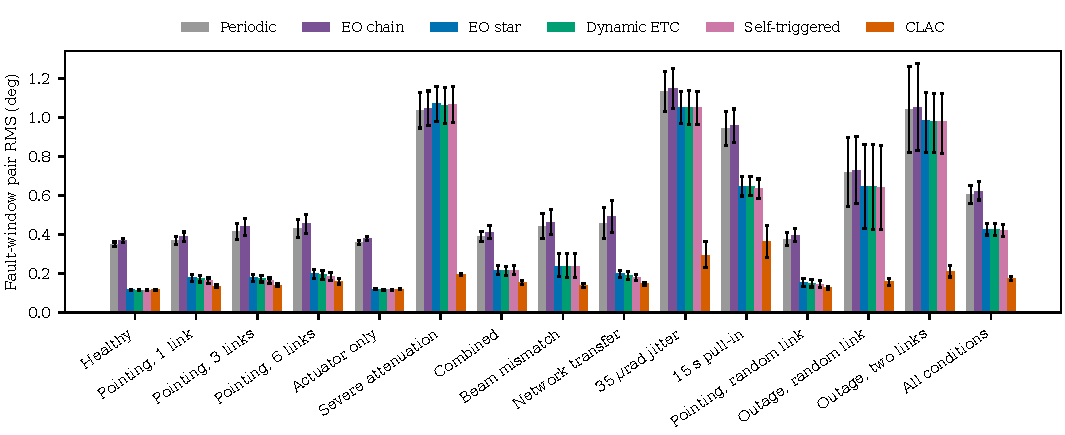
\includegraphics[width=\textwidth]{figures/fig_v2_pair.pdf}
\caption{Fault-window pair RMS with 95\% bootstrap intervals (20 held-out seeds) for six methods in 14 conditions and their mean.}
\label{fig:pair}
\end{figure*}

\begin{table*}[!t]
\caption{CLAC minus baseline: paired change in pair RMS (\%), mean [95\% CI]. Negative values favour CLAC.}
\label{tab:contrast}
\centering\scriptsize
\begin{tabular}{@{}lrrrr@{}}
\toprule
Condition & vs EO star & vs DET & vs ST & vs CLAC-fixed\\
\midrule
Healthy & 0.1 [-0.3, 0.7] & 1.8 [1.4, 2.4] & 2.3 [1.9, 2.9] & -67.4 [-67.9, -66.9]\\
Pointing, one link & -21.2 [-28.6, -13.6] & -19.5 [-27.0, -11.9] & -15.5 [-22.3, -8.6] & -64.9 [-66.3, -63.3]\\
Pointing, three links & -18.6 [-24.6, -12.4] & -16.9 [-22.8, -10.6] & -12.7 [-17.7, -7.3] & -65.6 [-67.3, -63.7]\\
Pointing, six links & -16.9 [-22.2, -11.0] & -14.8 [-19.5, -9.3] & -10.9 [-15.3, -6.0] & -62.1 [-63.8, -60.3]\\
Actuator only & 0.1 [-0.3, 0.7] & 1.8 [1.4, 2.4] & 2.3 [1.9, 2.9] & -67.6 [-68.1, -67.1]\\
Severe attenuation & -81.1 [-82.6, -79.6] & -81.0 [-82.5, -79.4] & -81.0 [-82.6, -79.4] & -80.3 [-82.0, -78.5]\\
Combined & -25.7 [-34.0, -17.0] & -23.9 [-32.4, -15.2] & -25.4 [-33.7, -16.8] & -60.8 [-64.3, -56.9]\\
Beam mismatch & -29.4 [-40.3, -19.0] & -28.2 [-39.5, -17.5] & -27.6 [-39.0, -16.8] & -67.5 [-71.3, -64.0]\\
Network transfer & -23.0 [-30.0, -15.8] & -19.3 [-27.0, -11.3] & -15.3 [-22.4, -8.1] & -56.7 [-62.1, -51.1]\\
35~$\mu$rad jitter & -71.2 [-77.3, -64.1] & -71.1 [-77.2, -64.0] & -71.1 [-77.1, -64.1] & -72.0 [-78.2, -64.8]\\
15~s pull-in & -42.6 [-55.3, -29.8] & -43.0 [-55.3, -30.6] & -41.7 [-54.5, -28.7] & -59.1 [-70.2, -47.8]\\
Pointing, random link & -11.5 [-19.4, -4.3] & -10.3 [-18.5, -2.7] & -8.4 [-16.0, -1.5] & -65.8 [-68.6, -63.3]\\
Outage, random link & -44.9 [-61.9, -27.9] & -44.1 [-61.4, -26.8] & -43.8 [-61.3, -26.4] & -69.1 [-76.9, -60.9]\\
Outage, two links & -71.4 [-80.5, -59.2] & -71.1 [-80.4, -58.7] & -71.0 [-80.3, -58.4] & -70.5 [-79.5, -60.3]\\
\midrule
Mean of 14 conditions & -58.4 [-61.2, -55.8] & -58.1 [-60.9, -55.4] & -57.6 [-60.5, -55.0] & -70.3 [-72.7, -67.7]\\
\bottomrule
\end{tabular}

\end{table*}

Three results stand out.
\emph{(i) Without a link fault, CLAC ties the best baseline.} In the healthy and isolated-actuator conditions CLAC differs from EO star by $+0.1\%$ (95\% CI: $[-0.3,0.7]\%$) and is $1.8$--$2.3\%$ worse than DET and ST. All three exploit a leader-fed star; the chain methods (EO chain, periodic, CLAC-fixed) are about 3 times worse because lag accumulates over three hops.
\emph{(ii) Under link faults CLAC wins by a wide margin.} Averaged over the 14 conditions, CLAC is 58.4\% lower than EO star (95\% CI: $[55.8, 61.2]\%$), 58.1\% lower than DET and 57.6\% lower than ST. Under severe attenuation of link 1--2 the star and chain methods stay at about 1.05$^\circ$ while CLAC reaches $0.195^\circ$ (81\% lower than EO star, CI $[79.6, 82.6]\%$) by routing SC2 through SC3 or SC4. Under random single-link outage the reduction against EO star is 44.9\% (CI: $[27.9, 61.9]\%$), and against two-link outage 71.4\% (CI: $[59.2, 80.5]\%$). Fig.~\ref{fig:trace} shows an outage of the SC1--SC4 link: SC4's error under the static star rises to about 2$^\circ$, and SC4 under CLAC moves to SC2, then SC3, and returns to SC1 after the link re-locks.
\emph{(iii) Pointing bias alone is mostly absorbed by recovery.} With one, three or six biased links the gains over EO star are $21.2\%$, $18.6\%$ and $16.9\%$ (CIs exclude zero). Going from one to three or six biased links raises the pair RMS of EO star and CLAC by 0.00--0.03$^\circ$ and of the chain methods by up to 0.07$^\circ$, so the earlier single-link concentration did not hide a large weakness of pilot recovery in this model.

\emph{Isolated actuator fault.} The actuator-only condition changes ideal-communication pair RMS from 0.333$^\circ$ to 0.343$^\circ$ and CLAC from 0.116$^\circ$ to 0.119$^\circ$. With effectiveness $0.30/0.45/0.35$, comparable to the actuator part of the combined condition ($0.25/0.40/0.30$), the feedback and disturbance estimator absorb the fault almost completely; the extra error of the combined condition therefore comes mainly from its optical components. A harsher actuator fault was not tested.

\emph{Stress cases.} Higher jitter (35~$\mu$rad) and slower acquisition (15~s) hurt every method; CLAC is 71\% lower than EO star under jitter (CI $[64.1, 77.3]\%$) and 43\% lower under slow acquisition (CI $[29.8, 55.3]\%$), but its pair RMS rises to $0.293^\circ$ and $0.363^\circ$, well above its other conditions.

\begin{figure}[!t]
\centering
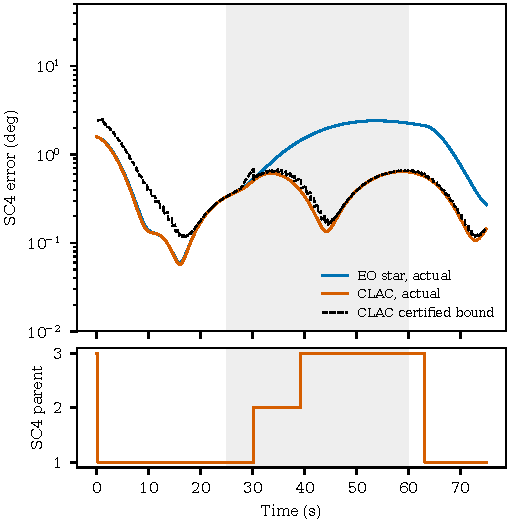
\includegraphics[width=\columnwidth]{figures/fig_v2_trace.pdf}
\caption{SC4 error and CLAC parent choice when the SC1--SC4 link is out (shaded; seed 203). The dashed line is the certified bound; the actual error never exceeds it.}
\label{fig:trace}
\end{figure}

\subsection{Communication Cost}
Table~\ref{tab:cost} and Fig.~\ref{fig:tradeoff} give mean payload. CLAC sends 78.6~kB (893 packets of 88~B), 14.5\% more than EO star (CI $[12.7,16.2]\%$), 8.9\% more than ST (CI $[6.9,10.7]\%$) and 9.6\% more than DET, and 45.4\% less than periodic exchange. The extra cost is the 24~B certificate and parent fields, upstream reports and standby heartbeats. CLAC without re-selection sends only 49.1~kB but has no advantage over the chain, so the gain comes from the combination of certificate and re-selection, not from the certificate alone.

\begin{table}[!t]
\caption{Mean over the 14 conditions: payload, attempted packets and pair RMS with 95\% CI.}
\label{tab:cost}
\centering\footnotesize
\begin{tabular}{@{}lrrr@{}}
\toprule
Method & Payload (kB) & Attempts & Pair RMS (deg)\\
\midrule
Ideal communication & 144.0 & 2250 & 0.326 [0.319, 0.334]\\
Periodic & 144.0 & 2250 & 0.604 [0.559, 0.650]\\
EO, chain & 82.6 & 1291 & 0.622 [0.576, 0.670]\\
EO, star & 68.8 & 1076 & 0.428 [0.397, 0.457]\\
Static ETC (ZOH) & 74.3 & 1162 & 0.622 [0.599, 0.643]\\
Dynamic ETC & 71.7 & 1120 & 0.424 [0.393, 0.454]\\
Self-triggered & 72.2 & 1128 & 0.420 [0.390, 0.450]\\
CLAC, no re-selection & 49.1 & 558 & 0.604 [0.557, 0.651]\\
CLAC & 78.6 & 893 & 0.175 [0.165, 0.185]\\
\bottomrule
\end{tabular}

\end{table}

\begin{figure}[!t]
\centering
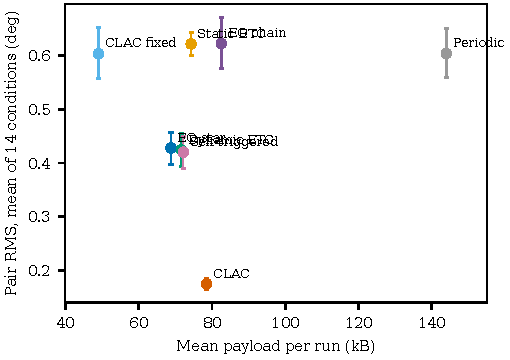
\includegraphics[width=\columnwidth]{figures/fig_v2_tradeoff.pdf}
\caption{Accuracy versus payload (mean of 14 conditions, 95\% interval on pair RMS).}
\label{fig:tradeoff}
\end{figure}

\subsection{Certificate Soundness}
The held-out runs contain 560 CLAC and CLAC-fixed runs. The actual attitude error never exceeded the certified bound at any of $1.5\times10^3$ samples per run (0 violations), including every outage condition. The bound is often tight: over CLAC runs the median of the per-run median ratio of actual to certified error is 0.95. The ratio is high because the bound adds the exact local tracking error to the extrapolation bound, and the local term dominates when messages are fresh; the bound is therefore informative about stale information only through its growth with age. CLAC switched parent on average 4.3 times per run (maximum 10).

\section{Discussion}
\emph{What the certificate buys.} The ablation shows that the certified horizon alone does not help: CLAC-fixed has the same pair RMS as periodic exchange on average (0.604$^\circ$), because a chain whose link fails has nobody else to listen to. The benefit appears when the bound is used to compare neighbours, which needs a bound that is valid regardless of which neighbour produced the packet. This is where the theorem matters: it licenses comparing candidates by their carried bounds without a model of the other spacecraft's controller.

\emph{Comparison with static trees.} A leader-fed star is as accurate as CLAC when nothing fails, and the baselines are tuned to the same payload, so the advantage of CLAC is specific to link faults. A designer who knew which link would fail could choose a tree that avoids it; CLAC does this online and without that knowledge, at 8.9--14.5\% more payload.

\emph{Why ideal communication is not a lower bound.} On the chain, ideal delivery gives $0.326^\circ$ because lag accumulates over three hops, while star-based methods reach $0.116^\circ$ when healthy. Calling ``ideal'' a bound would be wrong; it is the same chain with perfect delivery.

\section{Limitations and Threats to Validity}\label{sec:limits}
\begin{itemize}
\item \textbf{Closed-loop stability is not proved.} Theorem~\ref{thm:cert} bounds the target error and, through the measured local error, the state error. It does not show that the local error stays bounded under delay, saturation and switching.
\item \textbf{The command class is assumed known} (Assumption~\ref{as:ref}); a wrong $\bar\omega$ or $\bar\alpha$ would break the certificate. The tightness of the bound is not claimed beyond what the certificate-soundness subsection reports.
\item \textbf{Data.} Only published TBIRD values calibrate the model; raw NASA telemetry is not public and no ISRO data were found. TBIRD is a 930~km downlink; the 1~km crosslink geometry, receiver, code and lock thresholds are modelled. No hardware-in-the-loop or independent high-fidelity simulator was used; the validation is of the link-budget arithmetic and of the code by tests, not of the whole system.
\item \textbf{Baselines are adaptations}, tuned with one parameter on development seeds. Other tuning or stronger triggering designs could narrow the gaps; the faulty-link conditions favour any method that can change its tree.
\item \textbf{Novelty} is stated relative to the literature we reviewed; absence of prior work cannot be proved.
\item \textbf{Scope.} Four spacecraft, fixed positions, a smooth sinusoidal command, 1~km range, one-way hidden fault injection; orbital dynamics, thermal effects and multi-hop routing are not modelled. The same simulator and a single author team produce the tuning and the evaluation.
\end{itemize}

\section{Conclusion}
A certificate that travels with the state and uses only the command-generator class turns neighbour selection into a computation the receiver can do on its own. In a physically modelled optical network CLAC matches the best budget-matched trigger when links work and cuts coordination error by about 58\% on average when they fail, at about 9--15\% more payload, and the certificate was never violated in 560 runs. What remains open is a closed-loop stability proof for the saturated delayed controller, validation with hardware or a separate high-fidelity simulator, and calibration with crosslink data when such data become public.

\section*{Data and Software Availability}
The code, configurations, tuning sweeps, lock file, result CSVs, analysis scripts and tests are in the project repository (\url{https://github.com/kaushalrog/Satellite-Optical-Fault-Recovery}, branch \texttt{ieee-transactions-revision}). MATLAB R2026a runs \texttt{run\_tests\_v2} and \texttt{run\_v2\_evaluation}; Python scripts regenerate all tables and figures. The NASA values come from the cited public reports.

\section*{Acknowledgment}
The authors thank the Amrita School of Artificial Intelligence for support.

\begin{thebibliography}{99}
\bibitem{click} NASA, ``CubeSat Laser Infrared CrosslinK (CLICK),'' NASA Small Spacecraft mission description, accessed Oct. 22, 2026. [Online]. Available: \url{https://www.nasa.gov/smallspacecraft/what-is-click/}
\bibitem{liu2018} G.-P. Liu and S. Zhang, ``A survey on formation control of small satellites,'' \emph{Proc. IEEE}, vol. 106, no. 3, pp. 440--457, 2018.
\bibitem{cai2014} H. Cai and J. Huang, ``The leader-following attitude control of multiple rigid spacecraft systems,'' \emph{Automatica}, vol. 50, no. 4, pp. 1109--1115, 2014.
\bibitem{wang2021} S. Wang, Z. Shu, and T. Chen, ``Event-triggered attitude synchronization of multiple rigid-body systems,'' \emph{Syst. Control Lett.}, vol. 149, p. 104879, 2021.
\bibitem{xie2023} X. Xie, T. Sheng, and X. Chen, ``Self-triggered formation control for multi-spacecraft attitude coordination with communication delays,'' \emph{J. Franklin Inst.}, vol. 360, no. 18, pp. 14696--14711, 2023.
\bibitem{xie2024asr} X. Xie, T. Sheng, and X. Chen, ``Self-triggered formation attitude control for multiple spacecraft with disturbances,'' \emph{Adv. Space Res.}, vol. 74, no. 3, pp. 1288--1299, 2024.
\bibitem{jia2023} Q. Jia, J. Gao, C. Zhang, C. K. Ahn, and D. Yu, ``Dynamic event-triggered attitude synchronization of multi-spacecraft formation via a learning neural network control approach,'' \emph{Aerosp. Sci. Technol.}, vol. 142, p. 108653, 2023.
\bibitem{xie2024taes} X. Xie, T. Sheng, and X. Chen, ``Dynamic event-triggered and self-triggered fault-tolerant attitude control for multiple spacecraft systems with uncertainties and input saturation,'' \emph{IEEE Trans. Aerosp. Electron. Syst.}, vol. 60, no. 3, pp. 2922--2933, Jun. 2024, doi: 10.1109/TAES.2024.3355381.
\bibitem{ren2007} W. Ren, ``Distributed attitude alignment in spacecraft formation flying,'' \emph{Int. J. Adapt. Control Signal Process.}, vol. 21, no. 2-3, pp. 95--113, 2007, doi: 10.1002/acs.916.
\bibitem{sarlette2009} A. Sarlette, R. Sepulchre, and N. E. Leonard, ``Autonomous rigid body attitude synchronization,'' \emph{Automatica}, vol. 45, no. 2, pp. 572--577, 2009, doi: 10.1016/j.automatica.2008.09.020.
\bibitem{abdessameud2009} A. Abdessameud and A. Tayebi, ``Attitude synchronization of a group of spacecraft without velocity measurements,'' \emph{IEEE Trans. Autom. Control}, vol. 54, no. 11, pp. 2642--2648, 2009, doi: 10.1109/TAC.2009.2031567.
\bibitem{mayhew2011} C. G. Mayhew, R. G. Sanfelice, and A. R. Teel, ``Quaternion-based hybrid control for robust global attitude tracking,'' \emph{IEEE Trans. Autom. Control}, vol. 56, no. 11, pp. 2555--2566, 2011, doi: 10.1109/TAC.2011.2108490.
\bibitem{dimarogonas2009} D. V. Dimarogonas, P. Tsiotras, and K. J. Kyriakopoulos, ``Leader--follower cooperative attitude control of multiple rigid bodies,'' \emph{Syst. Control Lett.}, vol. 58, no. 6, pp. 429--435, 2009.
\bibitem{tabuada2007} P. Tabuada, ``Event-triggered real-time scheduling of stabilizing control tasks,'' \emph{IEEE Trans. Autom. Control}, vol. 52, no. 9, pp. 1680--1685, 2007, doi: 10.1109/TAC.2007.904277.
\bibitem{girard2015} A. Girard, ``Dynamic triggering mechanisms for event-triggered control,'' \emph{IEEE Trans. Autom. Control}, vol. 60, no. 7, pp. 1992--1997, 2015, doi: 10.1109/TAC.2014.2366855.
\bibitem{heemels2012} W. Heemels, K. Johansson, and P. Tabuada, ``An introduction to event-triggered and self-triggered control,'' in \emph{Proc. 51st IEEE Conf. Decision Control (CDC)}, 2012, pp. 3270--3285.
\bibitem{nowzari2019} C. Nowzari, E. Garcia, and J. Cort\'es, ``Event-triggered communication and control of networked systems for multi-agent consensus,'' \emph{Automatica}, vol. 105, pp. 1--27, 2019, doi: 10.1016/j.automatica.2019.03.009.
\bibitem{heemels2013} W. P. M. H. Heemels, M. C. F. Donkers, and A. R. Teel, ``Periodic event-triggered control for linear systems,'' \emph{IEEE Trans. Autom. Control}, vol. 58, no. 4, pp. 847--861, 2013, doi: 10.1109/TAC.2012.2220443.
\bibitem{mazo2010} M. Mazo, Jr., A. Anta, and P. Tabuada, ``An ISS self-triggered implementation of linear controllers,'' \emph{Automatica}, vol. 46, no. 8, pp. 1310--1314, 2010, doi: 10.1016/j.automatica.2010.05.009.
\bibitem{donkers2012} M. C. F. Donkers and W. P. M. H. Heemels, ``Output-based event-triggered control with guaranteed $\mathcal{L}_\infty$-gain and improved and decentralized event-triggering,'' \emph{IEEE Trans. Autom. Control}, vol. 57, no. 6, pp. 1362--1376, 2012, doi: 10.1109/TAC.2011.2174696.
\bibitem{olfati2007} R. Olfati-Saber, J. A. Fax, and R. M. Murray, ``Consensus and cooperation in networked multi-agent systems,'' \emph{Proc. IEEE}, vol. 95, no. 1, pp. 215--233, 2007, doi: 10.1109/JPROC.2006.887293.
\bibitem{hespanha2007} J. P. Hespanha, P. Naghshtabrizi, and Y. Xu, ``A survey of recent results in networked control systems,'' \emph{Proc. IEEE}, vol. 95, no. 1, pp. 138--162, 2007.
\bibitem{zhang2001} W. Zhang, M. S. Branicky, and S. M. Phillips, ``Stability of networked control systems,'' \emph{IEEE Control Syst. Mag.}, vol. 21, no. 1, pp. 84--99, 2001, doi: 10.1109/37.898794.
\bibitem{sinopoli2004} B. Sinopoli, L. Schenato, M. Franceschetti, K. Poolla, M. I. Jordan, and S. S. Sastry, ``Kalman filtering with intermittent observations,'' \emph{IEEE Trans. Autom. Control}, vol. 49, no. 9, pp. 1453--1464, 2004, doi: 10.1109/TAC.2004.834121.
\bibitem{kaymak2018} Y. Kaymak, R. Rojas-Cessa, J. Feng, N. Ansari, M. Zhou, and T. Zhang, ``A survey on acquisition, tracking, and pointing mechanisms for mobile free-space optical communications,'' \emph{IEEE Commun. Surveys Tuts.}, vol. 20, no. 2, pp. 1104--1123, 2018.
\bibitem{kaushal2017} H. Kaushal and G. Kaddoum, ``Optical communication in space: Challenges and mitigation techniques,'' \emph{IEEE Commun. Surveys Tuts.}, vol. 19, no. 1, pp. 57--96, 2017.
\bibitem{toyoshima2005} M. Toyoshima, ``Trends in satellite communications and the role of optical free-space communications [Invited],'' \emph{J. Opt. Netw.}, vol. 4, no. 6, pp. 300--311, 2005, doi: 10.1364/JON.4.000300.
\bibitem{farid2007} A. A. Farid and S. Hranilovic, ``Outage capacity optimization for free-space optical links with pointing errors,'' \emph{J. Lightw. Technol.}, vol. 25, no. 7, pp. 1702--1710, 2007, doi: 10.1109/JLT.2007.899174.
\bibitem{khalighi2014} M. A. Khalighi and M. Uysal, ``Survey on free space optical communication: A communication theory perspective,'' \emph{IEEE Commun. Surveys Tuts.}, vol. 16, no. 4, pp. 2231--2258, 2014, doi: 10.1109/COMST.2014.2329501.
\bibitem{schieler2023} C. M. Schieler \emph{et al.}, ``On-orbit demonstration of 200-Gbps laser communication downlink from the TBIRD CubeSat,'' in \emph{Proc. SPIE}, 2023, NASA Tech. Rep. NTRS 20230000434. [Online]. Available: \url{https://ntrs.nasa.gov/citations/20230000434}
\bibitem{schieler2023icsos} C. M. Schieler \emph{et al.}, ``Recent on-orbit results and ARQ performance analysis for the TBIRD 200-Gbps mission,'' in \emph{Proc. Int. Conf. Space Opt. Syst. Appl. (ICSOS)}, 2023, NASA Tech. Rep. NTRS 20230014010. [Online]. Available: \url{https://ntrs.nasa.gov/citations/20230014010}
\bibitem{reed1960} I. S. Reed and G. Solomon, ``Polynomial codes over certain finite fields,'' \emph{J. Soc. Ind. Appl. Math.}, vol. 8, no. 2, pp. 300--304, 1960.
\bibitem{zhang2008} Y. Zhang and J. Jiang, ``Bibliographical review on reconfigurable fault-tolerant control systems,'' \emph{Annu. Rev. Control}, vol. 32, no. 2, pp. 229--252, 2008, doi: 10.1016/j.arcontrol.2008.03.008.
\bibitem{heirung2019} T. A. N. Heirung and A. Mesbah, ``Input design for active fault diagnosis,'' \emph{Annu. Rev. Control}, vol. 47, pp. 35--50, 2019, doi: 10.1016/j.arcontrol.2019.03.002.
\bibitem{scott2014} J. K. Scott, R. Findeisen, R. D. Braatz, and D. M. Raimondo, ``Input design for guaranteed fault diagnosis using zonotopes,'' \emph{Automatica}, vol. 50, no. 6, pp. 1580--1589, 2014, doi: 10.1016/j.automatica.2014.03.016.
\bibitem{raimondo2016} D. M. Raimondo, G. R. Marseglia, R. D. Braatz, and J. K. Scott, ``Closed-loop input design for guaranteed fault diagnosis using set-valued observers,'' \emph{Automatica}, vol. 74, pp. 107--117, 2016, doi: 10.1016/j.automatica.2016.07.033.
\end{thebibliography}
\end{document}
